\documentclass[semifinal]{cpecmu}

%% This is a sample document demonstrating how to use the CPECMU
%% project template. If you are having trouble, see "cpecmu.pdf" for
%% documentation.

\projectNo{S013-2}
\acadyear{2022}

\titleTH{เว็บแอปพลิเคชันสำหรับการค้นหาตำแหน่งที่นั่งที่ยังว่างอยู่ภายในสำนักหอสมุดมหาวิทยาลัยเชียงใหม่}
\titleEN{Web application to find available seats in the Chiang Mai University Library}

\author{นางสาว ชวัลลักษณ์  แก้วมูล}{Chawanluck Kaewmool}{620610783}
\author{นาย ธนดล ตระกูลขยัน}{Tanadol Takunkayan}{620610792}

\cpeadvisor{arnan}
\cpecommittee{dome}
\cpecommittee{lachana}
%% Some possible packages to include:
\usepackage[final]{graphicx} % for including graphics

%% Add bookmarks and hyperlinks in the document.
\PassOptionsToPackage{hyphens}{url}
\usepackage[colorlinks=true,allcolors=Blue4,citecolor=red,linktoc=all]{hyperref}
\def\UrlLeft#1\UrlRight{$#1$}

%% Needed just by this example, but maybe not by most reports
\usepackage{afterpage} % for outputting
\usepackage{pdflscape} % for landscape figures and tables. 

%% Some other useful packages. Look these up to find out how to use
%% them.
% \usepackage{natbib}    % for author-year citation styles
% \usepackage{txfonts}
% \usepackage{appendix}  % for appendices on a per-chapter basis
% \usepackage{xtab}      % for tables that go over multiple pages
% \usepackage{subfigure} % for subfigures within a figure
% \usepackage{pstricks,pdftricks} % for access to special PostScript and PDF commands
% \usepackage{nomencl}   % if you have a list of abbreviations

%% if you're having problems with overfull boxes, you may need to increase
%% the tolerance to 9999
% \tolerance=9999

\bibliographystyle{plain}
% \bibliographystyle{IEEEbib}

% \renewcommand{\topfraction}{0.85}
% \renewcommand{\textfraction}{0.1}
% \renewcommand{\floatpagefraction}{0.75}

%% Example for glossary entry
%% Need to use glossary option
%% See glossaries package for complete documentation.
\ifglossary
  \newglossaryentry{lorem ipsum}{
    name=lorem ipsum,
    description={derived from Latin dolorem ipsum, translated as ``pain itself''}
  }
\fi

%% Uncomment this command to preview only specified LaTeX file(s)
%% imported with \include command below.
%% Any other file imported via \include but not specified here will not
%% be previewed.
%% Useful if your report is large, as you might not want to build
%% the entire file when editing a certain part of your report.
% \includeonly{chapters/intro,chapters/background}

\begin{document}
\maketitle
\makesignature

\ifproject
\begin{abstractTH}
    โครงงานนี้เป็นการพัฒนาเว็บแอปพลิเคชันสำหรับการค้นหาตำแหน่งที่นั่งที่ยังว่างอยู่ 
    \enskip ภายในสำนักหอสมุดมหาวิทยาลัยเชียงใหม่ 
    เนื่องจากมีนักศึกษาเข้าใช้หอสมุดจำนวนมากโดยเฉพาะอย่างยิ่งในช่วงสอบ 
    หากใช้งานเว็บแอปพลิเคชันนี้จะทำให้สามารถรู้ตำแหน่งที่นั่งที่ยังว่างอยู่ล่วงหน้าก่อนเข้าใช้หอสมุดได้ 
    และไม่ต้องเสียเวลาในการเดินวนหาที่นั่งในแต่ละชั้น เพราะในเว็บแอปพลิเคชันนี้จะแสดงตำแหน่งที่นั่งที่ยังว่างอยู่
    \enskip ในแต่ละชั้นของหอสมุด จำนวนผู้ใช้งาน และจำนวนที่นั่งที่ยังว่างอยู่จากจำนวนที่นั่งทั้งหมดอีกด้วย 
    โดยจะมีการใช้ Machine Learning ทำ Camera Object Detection 
    ในการนับจำนวนคนและตรวจสอบที่นั่งที่ยังว่างอยู่จากกล้องวงจรปิดที่ทางสำนักหอสมุดได้ติดตั้งไว้ 
    แล้วจึงส่งข้อมูลที่ได้มาที่เว็บแอปพลิชันเพื่อแสดงผลให้แก่ผู้ใช้งานเว็บแอปพลิชันนี้    
\end{abstractTH}

\begin{abstract}
The abstract would be placed here. It usually does not exceed 350 words
long (not counting the heading), and must not take up more than one (1) page
(even if fewer than 350 words long).

Make sure your abstract sits inside the \texttt{abstract} environment.
\end{abstract}

\iffalse
\begin{dedication}
This document is dedicated to all Chiang Mai University students.

Dedication page is optional.
\end{dedication}
\fi % \iffalse

\begin{acknowledgments}
Your acknowledgments go here. Make sure it sits inside the
\texttt{acknowledgment} environment.

\acksign{2020}{5}{25}
\end{acknowledgments}%
\fi % \ifproject

\contentspage

\ifproject
\figurelistpage

\tablelistpage
\fi % \ifproject

% \abbrlist % this page is optional

% \symlist % this page is optional

% \preface % this section is optional


\pagestyle{empty}\cleardoublepage
\normalspacing \setcounter{page}{1} \pagenumbering{arabic} \pagestyle{cpecmu}

\chapter{\ifenglish Introduction\else บทนำ\fi}

\section{\ifenglish Project rationale\else ที่มาของโครงงาน\fi}
จากปัญหาที่ได้พบจากการสอบถามกับทางหอสมุดและคนรอบตัวที่ใช้บริการของหอสมุดเป็นประจำ พบว่าในแต่ละวันมีนักศึกษามหาวิทยาลัยเชียงใหม่มีจำนวนมากที่มาใช้หอสมุดโดยเฉพาะในช่วงสอบ แต่อาจไม่สามารถหาที่นั่งว่างได้ง่าย ๆ 
เพราะยังไม่มีระบบการแจ้งเตือนที่ช่วยบอกล่วงหน้าว่ามีที่นั่งว่างในหอสมุดหรือไม่ ทำให้ตัวนักศึกษาจำเป็นต้องเดินทางมาที่หอสมุดแล้วเดินหาที่ว่างเอง ทำให้เสียเวลาในการค้นหาและยังทำให้หอสมุดมีความแออัดโดยไม่จำเป็นอีกด้วย
ดังนั้น โครงงานนี้จึงช่วยแก้ไขปัญหาที่กล่าวมาโดยการพัฒนาเว็บแอปพลิเคชันที่ช่วยให้ผู้ใช้งานสามารถรู้ตำแหน่งที่นั่งว่างในหอสมุดได้ก่อนเข้าใช้บริการ ทำให้ผู้ใช้สามาวางแผนการหาสถานที่อ่านหนังสือได้ง่ายขึ้น 
และไม่เสียเวลาไปกับการหาที่นั่งที่ว่างอยู่ด้วย
\section{\ifenglish Objectives\else วัตถุประสงค์ของโครงงาน\fi}
\begin{enumerate}
    \item เพื่อให้ผู้ใช้งานหาที่นั่งได้ง่ายขึ้น
    \item เพื่อให้ผู้ใช้งานสามารถทราบล่วงหน้าว่ายังมีที่นั่งว่างเหลืออยู่หรือไม่ 
    \item เพื่อให้สำนักหอสมุดสามารถ บันทึกสถิติแล้วนำไปปรับปรุงหอสมุดให้ดีขึ้น
\end{enumerate}

\section{\ifenglish Project scope\else ขอบเขตของโครงงาน\fi}

\subsection{\ifenglish Hardware scope\else ขอบเขตด้านฮาร์ดแวร์\fi}
โมเดล จะมีการทำงานภายในสำนักหอสมุด มหาวิทยาลัยเชียงใหม่
\subsection{\ifenglish Software scope\else ขอบเขตด้านซอฟต์แวร์\fi}

\section{\ifenglish Expected outcomes\else ประโยชน์ที่ได้รับ\fi}

\section{\ifenglish Technology and tools\else เทคโนโลยีและเครื่องมือที่ใช้\fi}

\subsection{\ifenglish Hardware technology\else เทคโนโลยีด้านฮาร์ดแวร์\fi}
\begin{itemize}
    \item ESP32-CAM with OV2640
    \item Acer Nitro 5
    \item acer aspire 7
\end{itemize}
\subsection{\ifenglish Software technology\else เทคโนโลยีด้านซอฟต์แวร์\fi}
\begin{itemize}
    \item Figma
    \item Python
    \item MongoDB
    \item React
    \item Node.js
    \item Visual Studio Code
    \item OpenCV
    \item Tensorflow
    \item Arduino IDE    
\end{itemize}
\section{\ifenglish Project plan\else แผนการดำเนินงาน\fi}

\begin{plan}{11}{2022}{10}{2023}
    \planitem{11}{2022}{12}{2022}{ศึกษาค้นคว้าข้อมูลในการทำโครงงาน}
    \planitem{12}{2022}{2}{2023}{ทดสอบการทำงานของ model ที่เลือกใช้}
    \planitem{2}{2023}{3}{2023}{เขียนรายงานและเตรียมนำเสนอ}
    \planitem{4}{2023}{6}{2023}{ออกแบบ Web Application}
    \planitem{6}{2023}{7}{2023}{ทดสอบการทำงานของ Web Application และติดตั้งอุปกรณ์}
    \planitem{8}{2023}{9}{2023}{ปรับปรุงและพัฒนาโครงงานให้ดีขึ้น}
    \planitem{9}{2023}{10}{2023}{สรุปผล ทำรายงาน และเตรียมนำเสนอ}
\end{plan}

\section{\ifenglish Roles and responsibilities\else บทบาทและความรับผิดชอบ\fi}
\begin{itemize}
\item ส่วนที่ทำงานร่วมกัน ได้แก่ การวางแผนการทำงาน การค้นหาข้อมูล และเครื่องมือ
\item ส่วนที่รับผิดชอบโดย นางสาว ชวัลลักษณ์ แก้วมูล ได้แก่ การพัฒนา
\item ส่วนที่รับผิดชอบโดย นาย ธนดล ตระกูลขยัน ได้แก่ การออกแบบ UI/UX ของระบบ และการพัฒนา Web application
\end{itemize}
\section{\ifenglish%
Impacts of this project on society, health, safety, legal, and cultural issues
\else%
ผลกระทบด้านสังคม สุขภาพ ความปลอดภัย กฎหมาย และวัฒนธรรม
\fi}
เขียนตรงนี้เพิ่มทีนะ

โครงงานเว็บแอปพลิเคชันสำหรับการค้นหาตำแหน่งที่นั่งที่ยังว่างอยู่ภายในสำนักหอสมุดมหาวิทยาลัยเชียงใหม่ เป็นโครงงานที่
นำการวิเคราะห์ของ Machine Learning เข้ามาช่วยในการ   ซึ่งจะช่วยประกอบการ
ตัดสินใจให้กับผู้ที่ โดยโครงงานได้คำนึงถึงกฎหมาย PDPA หรือ พ.ร.บ. คุ้มครองข้อมูลส่วนบุคคล ข้อมูลที่
โครงงานได้นำมาใช้วิเคราะห์นั้น 
ไม่ระบุตัวตน ซึ่งทำให้ไม่มีความกังวลที่ข้อมูลส่วนตัวจะ
ถูกเปิดเผย นอกจากนั้นโครงงานนี้ยังเป็น

\chapter{\ifenglish Background Knowledge and Theory\else ทฤษฎีที่เกี่ยวข้อง\fi}

ในบทนี้ก็จะเกี่ยวกับการอธิบายถึงสิ่งที่เกี่ยวข้องกับโครงงาน เพื่อให้ผู้อ่านเข้าใจเนื้อหาในบทถัดๆ ไปได้ง่ายขึ้น

\section{ด้าน Backend}
The text for Section 1 goes here.

\subsection{Computer Vision}

Subsection 1 text

\subsection{Machine Learning}
Subsubsection 1 text

\subsection{NoSQL Database}
Subsubsection 2 text

\subsection{RESTful API}
Subsubsection 2 text

\section{ด้าน Frontend}


\subsection{React}
    React เป็นไลบรารี JavaScript ที่ช่วยให้ผู้พัฒนาสามารถสร้าง User Interface (UI) ได้อย่างง่ายดายและมีประสิทธิภาพ โดย React เน้นการสร้าง UI ที่มีการอัปเดตสถานะ (state) 
และการใช้งาน Component ในการแบ่งแยกหน้าที่การแสดงผลออกจากโค้ดหลัก โดย React นั้นได้รับความนิยมเนื่องจากมีความยืดหยุ่นสูง รองรับการพัฒนาแอปพลิเคชันแบบ Single Page Application (SPA) 
และสามารถใช้งานร่วมกับไลบรารีและเครื่องมืออื่น ๆ ได้อย่างคล่องตัว
    React มีโครงสร้างหลัก 3 ส่วน คือ Element, Component และ JSX โดย Element เป็นตัวแทนของ Element ใน HTML สามารถสร้าง Element ได้โดยใช้ React.createElement() 
และ Component เป็นส่วนประกอบของ UI ที่มีการจัดการข้อมูลและการแสดงผลโดยเฉพาะ สามารถสร้าง Component ด้วยการสร้าง Class หรือ Function และ JSX เป็นการเขียนโค้ดของ React 
ที่ผสมผสานระหว่าง JavaScript และ HTML ซึ่งจะถูกแปลงเป็น JavaScript โดย Babel\cite{React}


\subsection{Authentication and Authorization}


\subsection{Authentication and Authorization}


\section{ด้าน Hardware}


\section{Alghorithm}





% define a command that produces some filler text, the lorem ipsum.


  % To include an image in the figure, say myimage.pdf, you could use
  % the following code. Look up the documentation for the package
  % graphicx for more information.
  % \includegraphics[width=\textwidth]{myimage}

% This code demonstrates how to get a landscape table or figure. It
% uses the package lscape to turn everything but the page number into
% landscape orientation. Everything should be included within an
% \afterpage{ .... } to avoid causing a page break too early.


\section{\ifenglish%
\ifcpe CPE \else ISNE \fi knowledge used, applied, or integrated in this project
\else%
ความรู้ตามหลักสูตรซึ่งถูกนำมาใช้หรือบูรณาการในโครงงาน
\fi
}

อธิบายถึงความรู้ และแนวทางการนำความรู้ต่างๆ ที่ได้เรียนตามหลักสูตร ซึ่งถูกนำมาใช้ในโครงงาน

\section{\ifenglish%
Extracurricular knowledge used, applied, or integrated in this project
\else%
ความรู้นอกหลักสูตรซึ่งถูกนำมาใช้หรือบูรณาการในโครงงาน
\fi
}

อธิบายถึงความรู้ต่างๆ ที่เรียนรู้ด้วยตนเอง และแนวทางการนำความรู้เหล่านั้นมาใช้ในโครงงาน

\chapter{\ifproject%
\ifenglish Project Structure and Methodology\else โครงสร้างและขั้นตอนการทำงาน\fi
\else%
\ifenglish Project Structure\else โครงสร้างของโครงงาน\fi
\fi
}

โครงสร้างและขั้นตอนการทำงานของโครงการนี้สามารถแบ่งเป็นหมวดหมู่ต่าง ๆ ได้ตามความเหมาะสมเพื่อความชัดเจนและความเข้าใจ โดยโครงสร้างของโปรเจ็คจะประกอบไปด้วย 4 ส่วนหลัก ได้แก่ Frontend, Backend, Hardware และ Configuration ซึ่งรายละเอียดของแต่ละส่วนมีดังนี้

\section{โครงสร้างของแอปพลิเคชัน}
\subsection{Frontend}
ประกอบไปด้วย โค้ด JavaScript, CSS, รูปภาพ, และไฟล์อื่น ๆ ของส่วนเว็บแอปพลิเคชัน
\subsection{ฺBackend}
ประกอบด้วยการเขียนโปรแกรมของ AWS Lambda Function เกี่ยวกับการเรียกใช้ API Gateway เพื่อรับ Request จาก frontend การส่งภาพจาก S3 ผ่าน AWS Rekognition เพื่อประมวลผลและส่งข้อมูลให้กับ Database
\subsection{ฺHardware}
ประกอบด้วยโค้ดสำหรับ ESP32-CAM ที่เขียนโดย Arduino IDE เพื่อให้ ESP32 ถ่ายภาพแลส่งข้อมูลไปยังระบบ AWS
\subsection{configuration}
รวมการกำหนดค่าต่าง ๆ ภายในระบบของ AWS และ credentials สำหรับการเข้าถึง AWS
\section{ขั้นตอนการทำงาน}
ขั้นตอนการทำงานเริ่มต้นจากการจับภาพจากกล้องบน ESP32-CAM จากนั้นภาพจะถูกส่งไปยังบริการ AWS S3 โดยเมื่อรูปภาพใหม่เข้าถึงใน S3 จะทำการเรียกใช้ฟังก์ชัน Lambda เพื่อใช้บริการ AWS Rekognition ในการประมลผล และส่งข้อมูลไปจัดเก็บที่ AWS DynamoDB ต่อ ซึ่งข้อมูลที่จัดเก็บใน DynamoDB จะถูกเรียกใช้โดยแอปพลิเคชันเว็บที่ deploy บน Vercel 
เว็บแอปพลิเคชันจะทำการสื่อสารกับ AWS ผ่าน AWS API Gateway เพื่อเรียกใช้งาน Lambda ในการดึงข้อมูลจากฐานข้อมูลและนำมาแสดงผลในเว็บแอปพลิเคชัน
\begin{figure}[h]
\centering
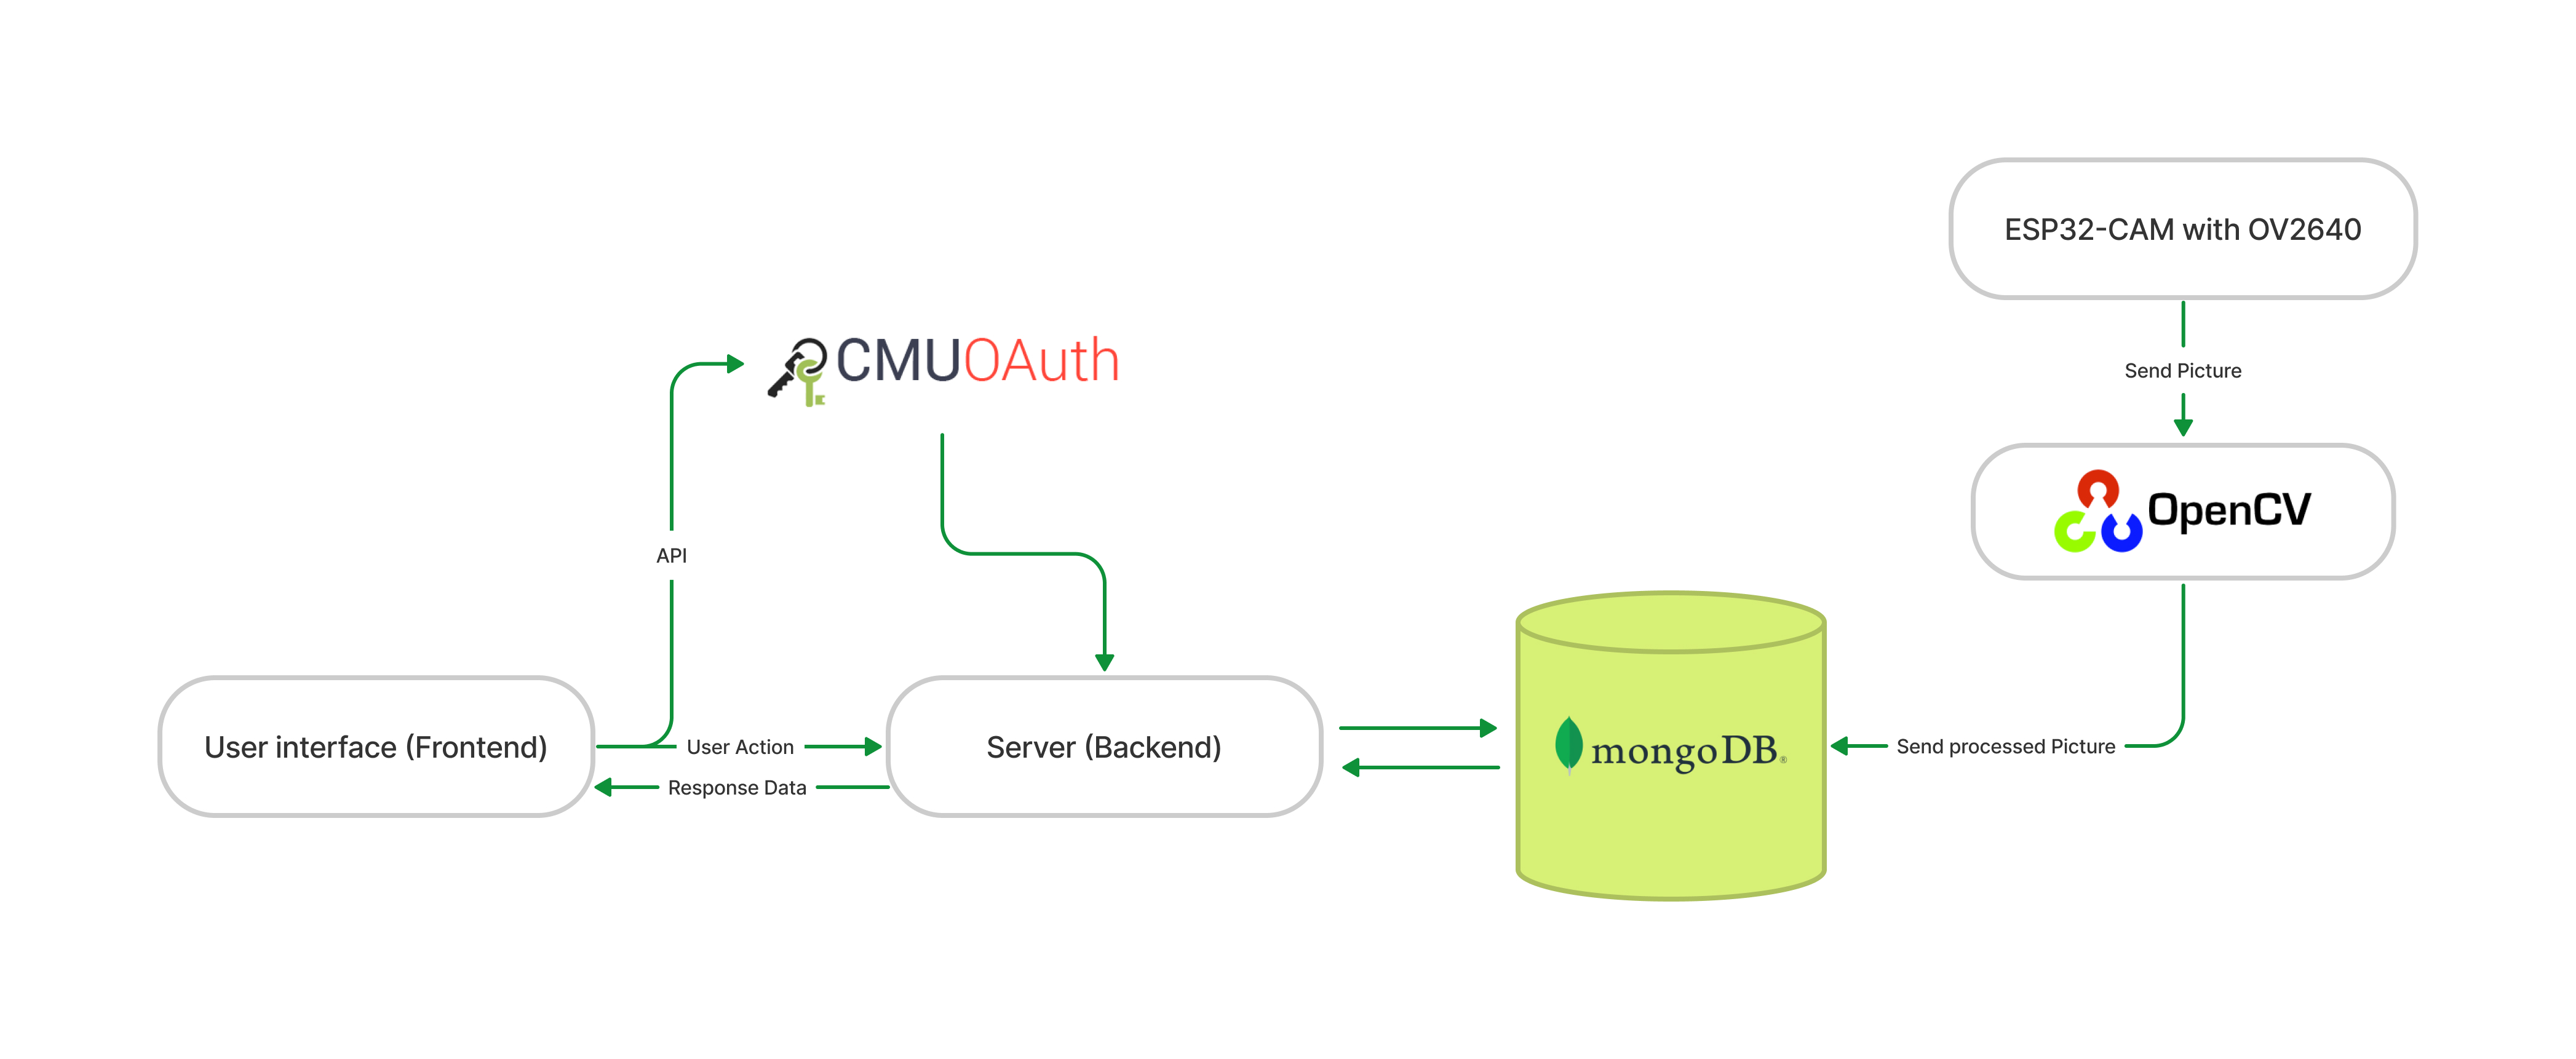
\includegraphics[width=\textwidth]{System Diagram.jpg}
\caption[System Overview]{System Overview}
\label{fig:System}
\end{figure}

\section{การใช้งานของแอปพลิเคชัน}
ผู้ใช้งานสามารถเข้าใช้งานตัวเว็บแอปพลิเคชันได้โดยไม่ต้องทำการล็อกอินหรือยืนยันตัวตน โดยสามารถเข้าถึงข้อมูลที่แสดงอยู่บน User Interface ได้แก่ จำนวนที่นั่งที่ยังว่างอยู่ จำนวนผู้เข้าใช้บริการในขณะนี้ 
และความหนาแน่นของผู้ใช้บริการหอสมุดในแต่ละช่วงเวลาย้อนหลัง


\chapter{\ifproject%
\ifenglish Experimentation and Results\else การทดลองและผลลัพธ์\fi
\else%
\ifenglish System Evaluation\else การประเมินระบบ\fi
\fi}

\hspace{10mm} เนื่องจากมีการนำความรู้เรื่อง Computer Vision มาใช้เกี่ยวกับการทำ Object detection จึงได้มีการศึกษา model และ library
ของ OpenCV ที่มีให้ทดลองใช้งาน เพื่อเพิ่มความเข้าใจและเลือกใช้ได้อย่างเหมาะสม โดยนำภาพบางส่วนจากการถ่ายรูปสถานที่จริงด้วยกล้องโทรศัพท์มือถือคือบริเวณชั้น 2
ของสำนักหอสมุดมหาวิทยาลัยเชียงใหม่มาทำการทดสอบ

\begin{figure}[h]
    \centering
    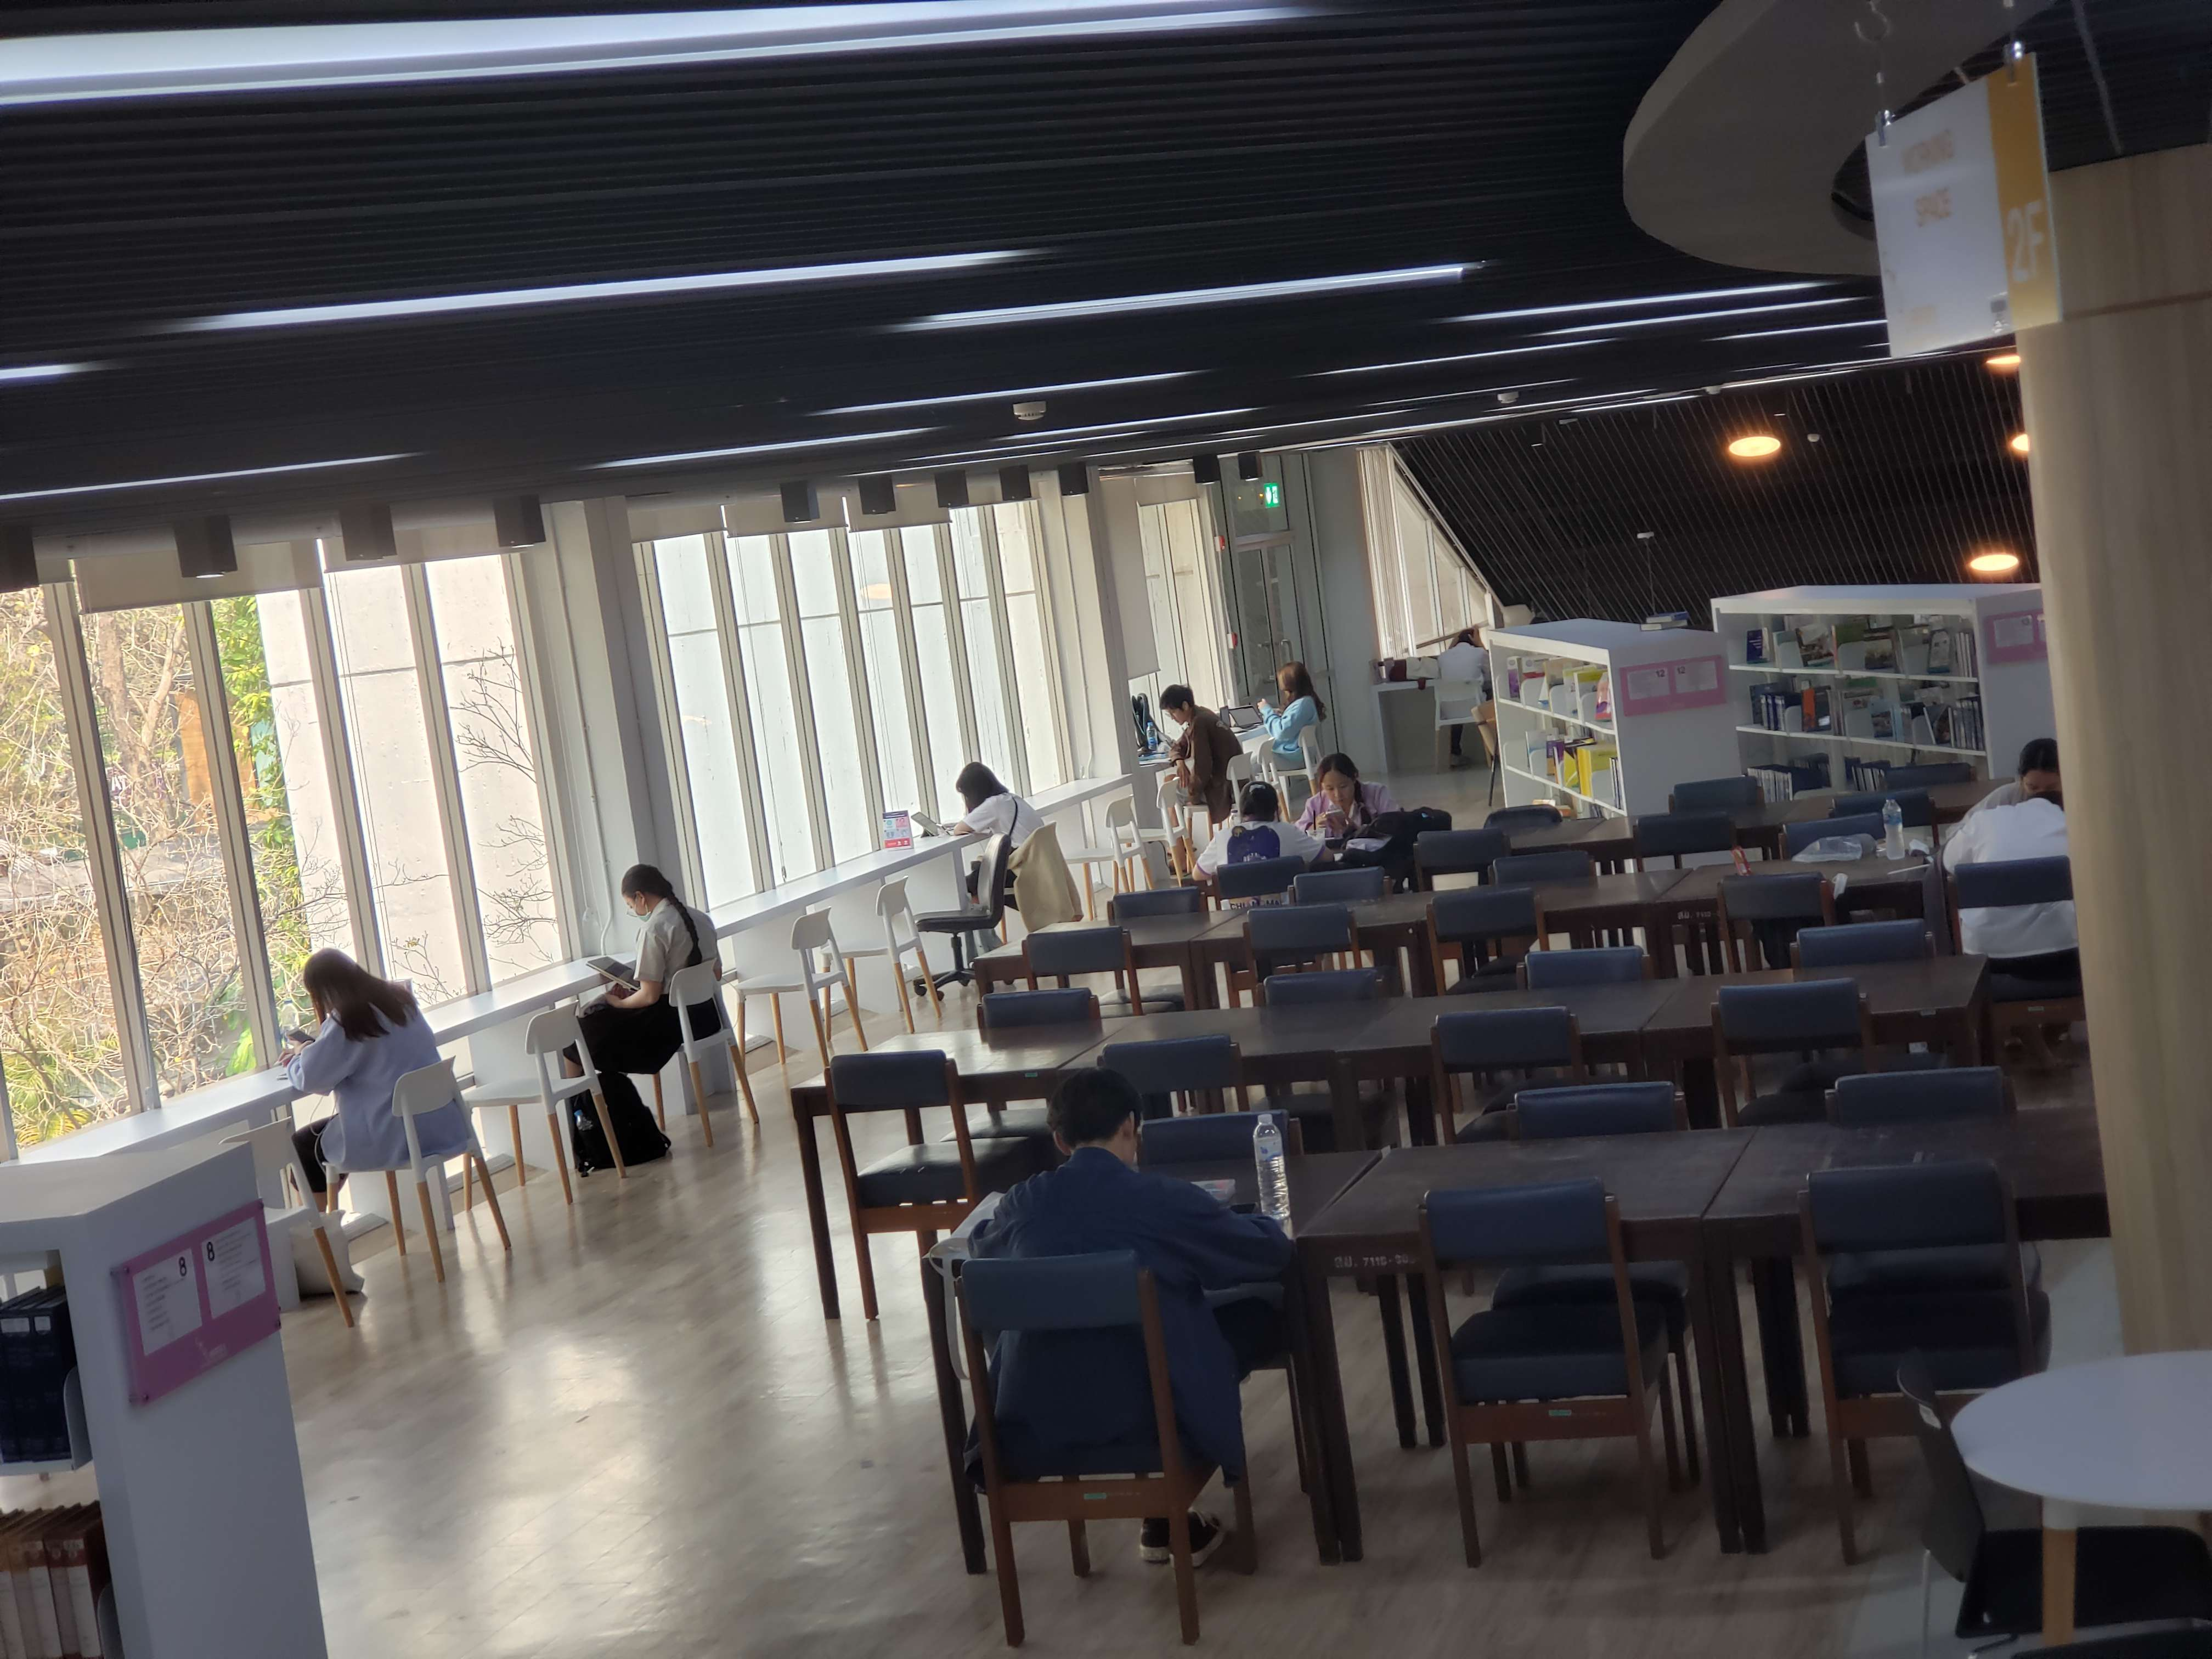
\includegraphics[scale=0.07]{images/cam2-2.jpg}
    \caption[camera]{ภาพจากกล้องโทรศัพท์มือถือ}
    \label{fig:camera}
\end{figure}

\section{การทดลองครั้งที่ 1 โดยใช้ OpenCV with HOG descriptor}
\begin{figure}[h]
    \centering
    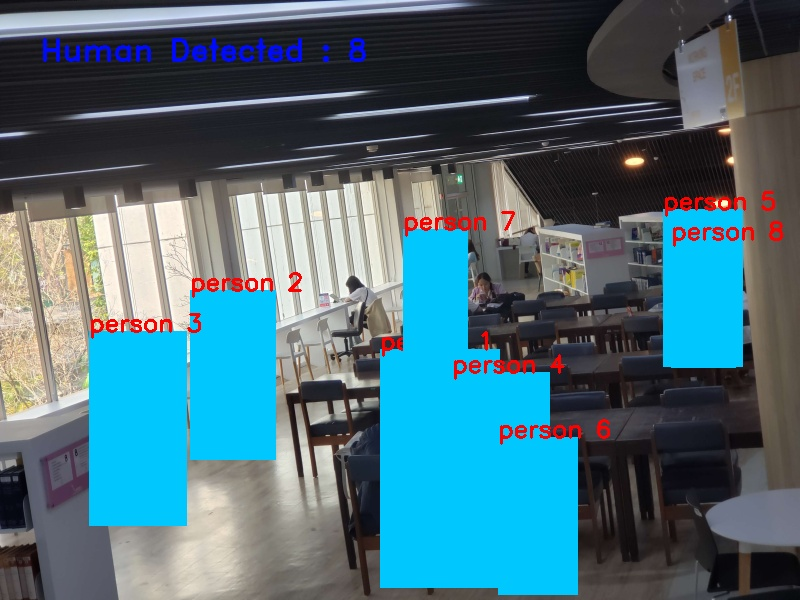
\includegraphics[scale=0.35]{images/hog_output.jpg}
    \caption[output]{output ของการทดลองครั้งที่ 1}
    \label{fig:output1}
\end{figure}

\section{การทดลองครั้งที่ 2 โดยใช้ OpenCV with Detect common object library}
\begin{figure}[h]
    \centering
    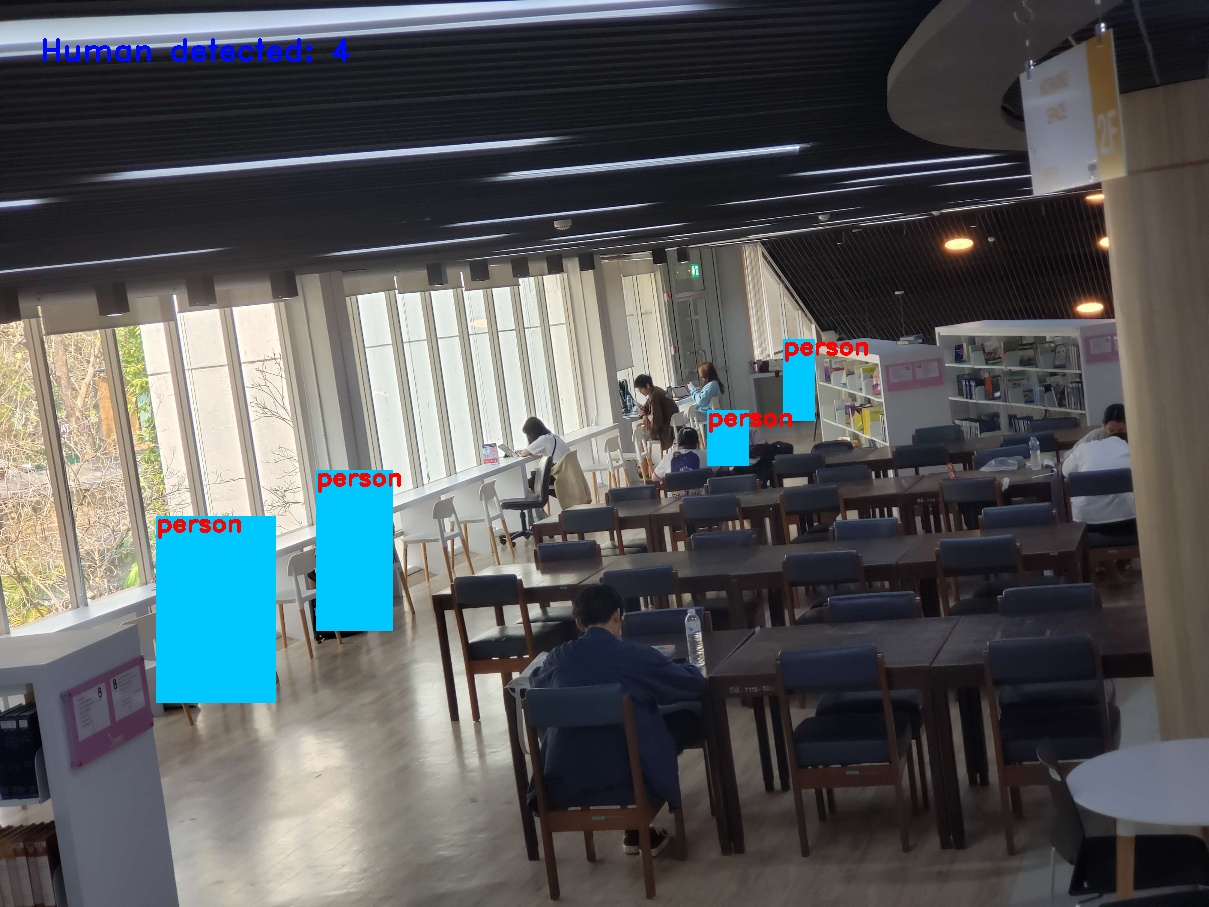
\includegraphics[scale=0.25]{images/cvlib_output.jpg}
    \caption[output]{output ของการทดลองครั้งที่ 2}
    \label{fig:output2}
\end{figure}

\section{การทดลองครั้งที่ 3 โดยใช้ OpenCV DNN with TensorFlow}
\begin{figure}[h]
    \centering
    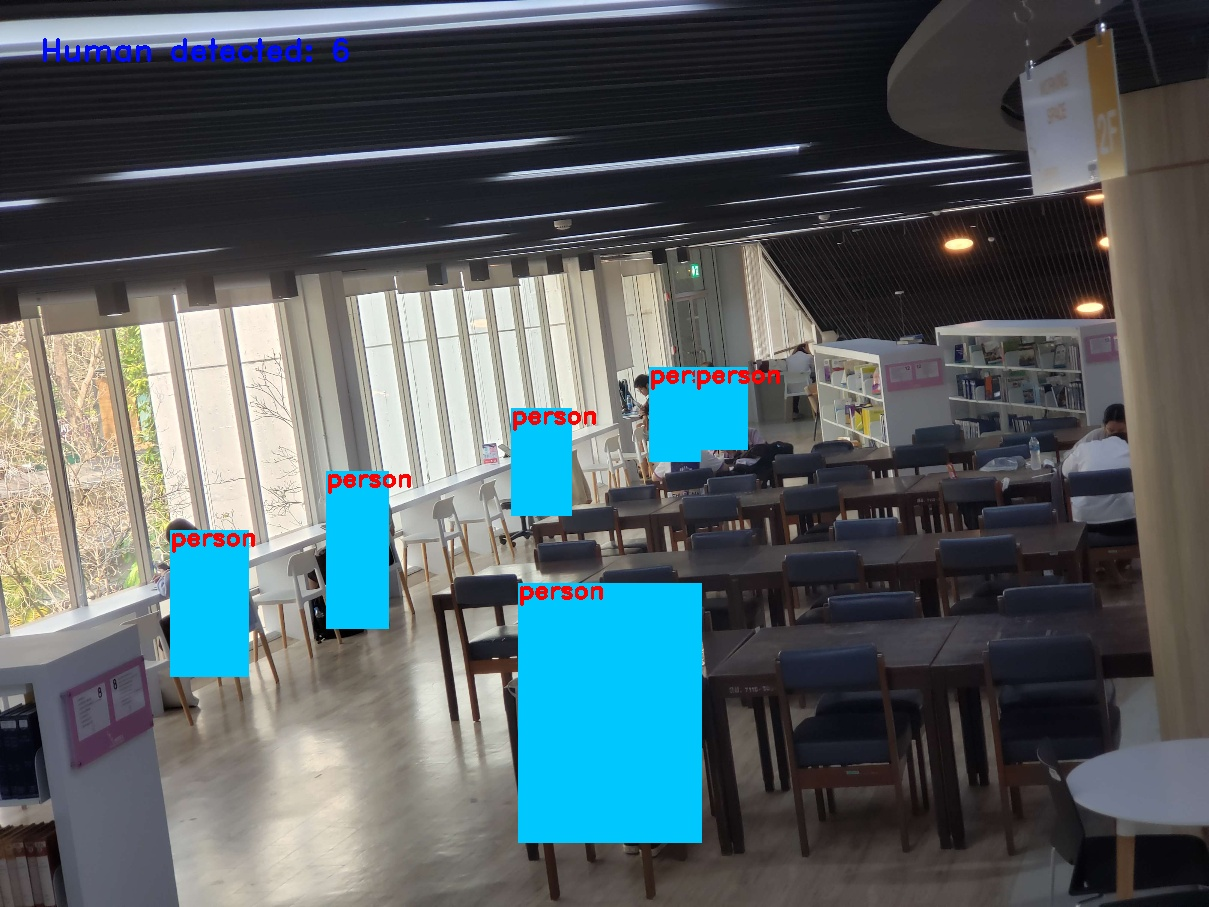
\includegraphics[scale=0.25]{images/dnn_output.jpg}
    \caption[output]{output ของการทดลองครั้งที่ 3}
    \label{fig:output3}
\end{figure}

\ifproject
\chapter{\ifenglish Conclusions and Discussions\else บทสรุปและข้อเสนอแนะ\fi}

\section{\ifenglish Conclusions\else สรุปผล\fi}

% นศ. ควรสรุปถึงข้อจำกัดของระบบในด้านต่างๆ ที่ระบบมีในเนื้อหาส่วนนี้ด้วย
จากผลการดำเนินงานนี้สามารถบรรลุวัตถุประสงค์ของโครงงานในการช่วยให้ผู้ใช้งานสามารถหาที่นั่งได้สะดวกมากยิ่งขึ้นและสามารถวางแผนล่วงหน้าได้ อีกทั้งผลประเมินความพึงพอใจโดยรวมเฉลี่ยถือว่าอยู่ในระดับที่ดี
แต่ยังมีข้อจำกัดในด้านของการแสดงผลที่ไม่ทั่วถึงเนื่องจากโครงงานนี้ทดสอบแค่ 3 โซนของบริเวณชั้น 2 ในสำนักหอสมุดมหาวิทยาลัยเชียงใหม่

\section{\ifenglish Challenges\else ปัญหาที่พบและแนวทางการแก้ไข\fi}

% ในการทำโครงงานนี้ พบว่าเกิดปัญหาหลักๆ ดังนี้
% \subsection{ในช่วงแรก ESP32-CAM with OV2640 ไม่สามารถส่งภาพไปยัง AWS S3 ได้}
% เนื่องจากยังไม่คุ้นชินกับการใช้ฟังก์ชันต่างๆ ของ AWS Web Service ทำให้ไม่สามารถส่งภาพจาก ESP32-CAM with OV2640 ได้ จึงแก้ไขให้ ESP32-CAM with OV2640 ส่งภาพไปเก็บไว้ที่ Google Drive ก่อนแล้วค่อย upload ไปยัง AWS S3 ทำให้การทำงานล่าช้าในช่วงแรกและซ้ำซ้อน 
% \subsection{ESP32-CAM with OV2640 ไม่สามารถเชื่อมต่อ WiFi ของ JumboPlus IoT ได้}
\begin{enumerate}
    \item ไม่สามารถ upload code ไปที่ ESP32-CAM with OV2640 ได้ ต้องทำการอัปเดต driver 
    \item ESP32-CAM with OV2640 ไม่สามารถเชื่อมต่อ WiFi ของ JumboPlus IoT ได้ จึงแก้ปัญหาโดยการแชร์ WiFi ของตนเองแทน
    \item ในช่วงแรก ESP32-CAM with OV2640 ไม่สามารถส่งภาพไปยัง AWS S3 ได้ เนื่องจากยังไม่คุ้นชินกับการใช้ฟังก์ชันต่างๆ ของ AWS Web Service 
    ทำให้ไม่สามารถส่งภาพจาก ESP32-CAM with OV2640 ได้ จึงแก้ไขให้ ESP32-CAM with OV2640 ส่งภาพไปเก็บไว้ที่ Google Drive ก่อนแล้วค่อย upload ไปยัง AWS S3 ทำให้การทำงานล่าช้าในช่วงแรกและซ้ำซ้อน
\end{enumerate}

\newpage
\section{\ifenglish%
Suggestions and further improvements
\else%
ข้อเสนอแนะและแนวทางการพัฒนาต่อ
\fi
}
% ข้อเสนอแนะเพื่อพัฒนาโครงงานนี้ต่อไป มีดังนี้
\subsection{ข้อเสนอแนะจากผู้ใช้งาน}
\begin{figure}[ht]
    \centering
    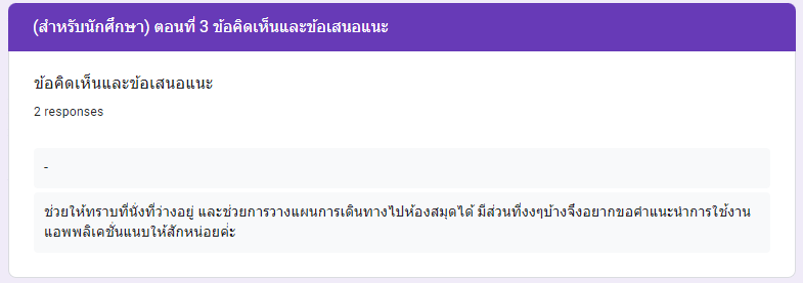
\includegraphics[scale=0.8]{images/student-s.png}
    \caption[st-s]{ข้อเสนอแนะจากนักศึกษา}
    \label{fig:st-s}
% \end{figure}
% \begin{figure}[ht]
    \centering
    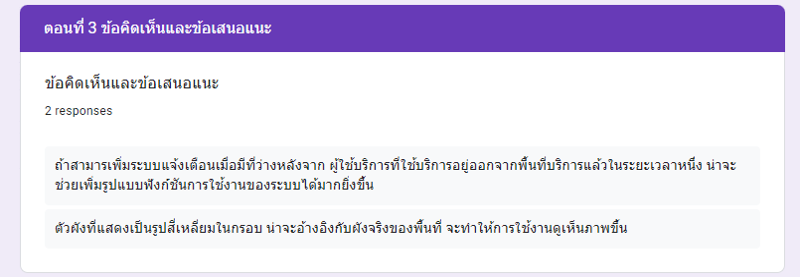
\includegraphics[scale=0.8]{images/cmul-s.png}
    \caption[cmul-s]{ข้อเสนอแนะจากทางสำนักหอสมุด}
    \label{fig:cmul-s}
\end{figure}

\subsection{ข้อเสนอแนะในการพัฒนาต่อ}
\subsection{ค่าใช้จ่ายในการพัฒนาต่อ}

\fi

\bibliography{sampleReport}

\ifproject
\normalspacing
\appendix
\include{chapters/appendix}

%% Display glossary (optional) -- need glossary option.
\ifglossary\glossarypage\fi

%% Display index (optional) -- need idx option.
\ifindex\indexpage\fi

\begin{biosketch}
\begin{center}
  \includegraphics[width=1.5in]{mugshot.jpg}
\end{center}
Your biosketch goes here. Make sure it sits inside
the \texttt{biosketch} environment.
\end{biosketch}
\fi % \ifproject
\end{document}
